\section{Introduction}
\subsection{Fidelity, Refinement, and Exploratory Extension (FiREE) Replication Framework}

A researcher faces at least two challenges when attempting to replicate previously published research: staying faithful to the original design while also ensuring that the replication is analytically robust and theoretically informative. Contemporary discussions in applied linguistics emphasize that replication is not simply about reproducing identical methods, but rather about maintaining core features of the original design while also correcting limitations and expanding interpretability \parencite{marsden2018,mcmanus2024,porte2018}. This paper contributes to that view by introducing the Fidelity, Refinement, and Exploratory Extension (FiREE) replication framework. FiREE integrates high-fidelity replication with methodological refinement and theory-driven exploratory analysis, providing a structured way to reproduce prior findings while also clarifying their robustness and generalizability.

Fidelity ensures the adherence to the original study design, using the same procedures and statistical models to assess whether the original findings hold under comparable conditions. Maintaining methodological consistency facilitates direct comparisons and contributes to broader efforts to establish replicability across fields. 

Refinement strengthens the analytical framework by incorporating improved statistical practices to address issues such as multiple comparisons, overfitting, and model complexity. This step ensures that any observed effects were not artifacts of less conservative analytical approaches. Moreover, this step ensures that effects were not overlooked due to less robust modeling approaches. Researchers must distinguish between effects that are method-dependent and those that hold across multiple different analytical choices.

Finally, exploratory extensions allow for the systematic examination of theoretical assumptions that may not have been explicitly tested in the original study. Exploratory extensions provide a structured, often theory-motivated examination of factors, such as individual differences, which may contribute to the results. This allows researchers to test established explanatory framework while generating new hypotheses to account for the variation. 

Our FiREE Replication approach encourages researchers to move beyond a binary success-or-failure replication framework \parencite{Nosek_Errington2020}. Instead, see it as an opportunity to evaluate methodological robustness, refine statistical practices, and uncover theoretical insights that were not explicitly addressed in the original research. This perspective frames replication as an active tool for scientific progress, reinforcing that replicability is not merely about reproducing a prior effect, but also about ensuring that findings are meaningful, interpretable, and generalizable across different statistical, methodological, and theoretical contexts.

While existing classifications such as exact, close, and conceptual replication describe the degree of similarity between original and replication studies \parencite{marsden2018, porte2018, mcmanus2024replication2}, the FiREE framework is concerned with the structure of \hl{methodological and analytical} choices in replication efforts—how researchers can combine fidelity, refinement, and exploratory extension in a single study. In this sense, FiREE is not a new replication type, but rather an orthogonal framework that encourages layered replication analysis design: a faithful reproduction of the original analysis (fidelity), followed by analytical improvements (refinement), and theoretically motivated additions (exploratory extension). That is, the FiREE framework could be applied to any replication regardless of degree of similarity. We view this as fully aligned with current thinking in applied psycholinguistics, particularly calls for transparency, theory-relevance, and statistical rigor in replication research. Moreover, as we demonstrate, the FiREE framework is a natural fit for behavioral and eye-tracking web-based studies.

In what follows, we first discuss the linguistic concept of focus and the findings of \textcite{ge2021a}---the focus processing eye-tracking study that we set out to closely replicate \parencite[see figure 1 of replication classification types][]{mcmanus2024replication2}. We then briefly review the acoustics of focus and five areas in which individuals differ in their language processing behavior. These acoustic cues and individual differences measures serve as predictors in the exploratory extension. We make all our methods, materials, code, and data freely available on the Open Science Framework. Using our \textcite{ge2021a} replication results, we demonstrate our FiREE framework and connect our replication and extension findings to larger theories of psycholinguistics and second language acquisition. 

\subsection{Focus in English \textit{only}-sentences}

Information in languages must be organized and presented in a manner that clearly and effectively conveys the speaker's intention. The study of how information is structured in language encompasses syntax, semantics, pragmatics, and prosody \parencite[see][] {Breen2010, Lambrecht1994, Roberts2012}. An important area of information structure is focus or the information that is considered most important, relevant, new or contrastive \parencite{Kiss1998}. Focus is believed to be a linguistic universal \parencite{Comrie1989}. How focus is implemented, however, varies across languages and can be constrained by a language’s phonology and morphosyntax \parencite{Kiss1998, Lambrecht1994}. That is, focus involves multiple levels of linguistic knowledge or interfaces. How speakers process focus in sentences is a rich area of psycholinguistics research \parencite[e.g.,][] {Cutler1979, Filik2005, Wang2011}. 

English realizes focus primarily through prosodic prominence—typically, a pitch accent on the focused constituent. This is especially clear in English sentences containing the focus-sensitive particle \textit{only}, which plays a central role in theoretical and experimental work on focus processing. In such sentences, the semantic scope of \textit{only} is often ambiguous and must be resolved through prosodic cues. As an example, take the sentence, “Obama only vetoed the bill.” The scope of the focus particle \textit{only} can be associated with the verb ‘vetoed’ or the object ‘the bill.’ Semantic parsing, however, depends on which word(s) carries prosodic prominence. If ‘the bill’ carries prosodic prominence, the listener will understand that Obama vetoed nothing else but the bill. In contrast, if ‘vetoed’ carries prosodic prominence, the listener will understand that Obama did nothing else to the bill other than veto it.

In the present study, we “focus” on English preverbal \textit{only}-sentences with varying positions of prosodic prominence because they offer a highly controlled paradigm for testing prosodic focus processing. Moreover, the ambiguity inherent in these sentences allows us to manipulate focus structure independently of word order or lexical content, providing a clean test case for examining interface processing—how syntax, semantics, and prosody are integrated in real time. This is particularly valuable in second language (L2) research, where learners may struggle to integrate multiple cues across linguistic domains.

\textcite{ge2021a}---the study we set out to closely replicate---examined how L1 and L2 English speakers process \textit{only}-sentences in real time. The authors used the “look-and-listen” visual world paradigm in which a participant looks at images on screen while listening to spoken sentences. Importantly, the images on the screen represented the intended target of the focus or the alternative focus (i.e., a competitor). For example, each experimental sentence stimulus contained \textit{only} with prosodic prominence on either the verb or the object, creating two conditions as in “The dinosaur is only CARRYING the bucket, not throwing the bucket” (verb condition; capital letters denote prominence) or “The dinosaur is only carrying the BUCKET, not carrying the suitcase” (object condition).

\textcite{ge2021a} tested L1 English speakers and L2 English learners whose L1 was either Cantonese or Dutch. Dutch, like English, uses prosodic prominence to realize focus through an expanded F0 range, increased amplitude, and longer durations \parencite{dimitrova2010focus}. Dutch \textit{only}-sentences (or \textit{alleen}-sentences, the Dutch equivalent) can pattern like English \textit{only}-sentences as in “De dinosaurus draagt alleen De EMMER” (The dinosaur is only carrying the BUCKET). Importantly, Dutch \textit{alleen}-sentences can also place \textit{only} after the object as in “De dinosaurus DRAAGT De emmer alleen” (The dinosaur is only CARRYING the bucket). In contrast, Cantonese \textit{only}-sentences are considerably different from those in English (and Dutch). Cantonese has a number of different focus particles, which makes prosody somewhat optional for realizing focus \parencite{lee2019focus, wu2010prosodic, ge2024bilingual, fung2000final}. 

The authors predicted that the presence of \textit{only} would prompt participants to search for the picture that depicts a focus alternative. That is, participants' looks to the on-screen images would diverge once focus prosodic information was integrated with semantic and syntactic information. For example, upon hearing object-focused trials (e.g., “...only carrying the BUCKET, not carrying the suitcase”), participants would first look to the object (i.e., the bucket) and then look to the alternative (i.e., the suitcase) upon hearing \textit{not}. \textcite{ge2021a} found L1 English speakers considered the alternative of focus at an early stage (generally before hearing “not” in sentences). L2 speakers showed delayed eye movements to the alternative of focus (generally while or after hearing “not” in sentences), with the L1 Dutch speakers showing even more delayed behavior than the L1 Cantonese speakers. The authors interpreted these differences as evidence for problematic integration of multiple interfaces (e.g., syntax-semantics, syntax-pragmatics) in real time. They connected their findings to the Prosodic-Learning Interference Hypothesis \parencite{tremblay2016effects, tremblay2021re}, which states that L2 learning of prosodic cues is more difficult when the L1 and L2 use similar prosodic cues as in Dutch-English and less difficult when the L1 and L2 use different prosodic cues as in Cantonese-English, which also uses spoken particles as cues \parencite[see also][]{ge2021b}. 

This finding was partially replicated and extended by \textcite{jansen2023influence} who tested a new set of L1 Dutch-L2 English speakers and found that L2 learners with a stronger musical pitch perception ability were more likely to fixate on the target and less likely to fixate on the competitor. Thus, not only does the L1 affect L2 prosody acquisition, but also individuals' perceptual abilities can play a role in L2 prosody acquisition.

We set out to \hl{closely} replicate \textcite{ge2021a} using web-based eye-tracking and open materials and code. We collected L1 English and L1 Dutch data but not L1 Cantonese data given current geopolitical constraints. We also measure and test the acoustics of the stimuli and multiple individual differences to determine what acoustic cues and behavioral measures, if any, serve as reliable predictors of focus processing in an L1 and L2. We selected \textcite{ge2021a} for replication due to the recency and theoretical relevance of its findings, particularly the unexpected delays observed in Dutch L2 English learners. The study also offered a strong foundation for exploring individual differences, making it well-suited for extension through acoustic validation and learner-level predictors within the FiREE framework.

\subsection{The acoustics of focus}
In order for a word to be prominent, it must be realized with one or more acoustic correlates that increase or enhance its perceptibility. A speaker generally does this through F0, amplitude, duration, i.e., nuclear pitch accent on the focal element(s) \parencite{Gussenhoven1983}. Speakers reliably mark focused words with a higher mean and max F0 (pitch), greater intensity (loudness), and longer durations than words not focused \parencite{Breen2010}.
With respect to the stimuli \textcite{ge2021a} created, the authors reported two significant duration differences: verb duration is longer in verb-focused condition than in object-focused condition; object duration is longer in object-focused condition than in verb-focused condition. No F0 or amplitude differences were reported. Presumably these acoustic cues contribute to eye movements. In our exploratory extension, we place an emphasis on linking variable input to eye movements to strengthen theory \parencite{magnuson2019fixations}. 

For example, Figure \ref{fig:acoustic} plots the F0 contours of the stimuli by condition (color) with time on the x-axis. For verb-focused sentences (indicated in orange), we see an increase in F0 at the “verb1” time bin and for object-focused sentences (indicated in blue), we see an increase in F0 at the “object1” time bin. F0 information is dynamic and unfolds over time. We assume all listeners are sensitive to this information and therefore ask (EE1) how do acoustic cues predict  participants' eye movements? We expect findings in line with what we know about the acoustics of information structure \parencite{Breen2010}.

\begin{figure}[H]  % 'p' puts it on its own page
    \centering
    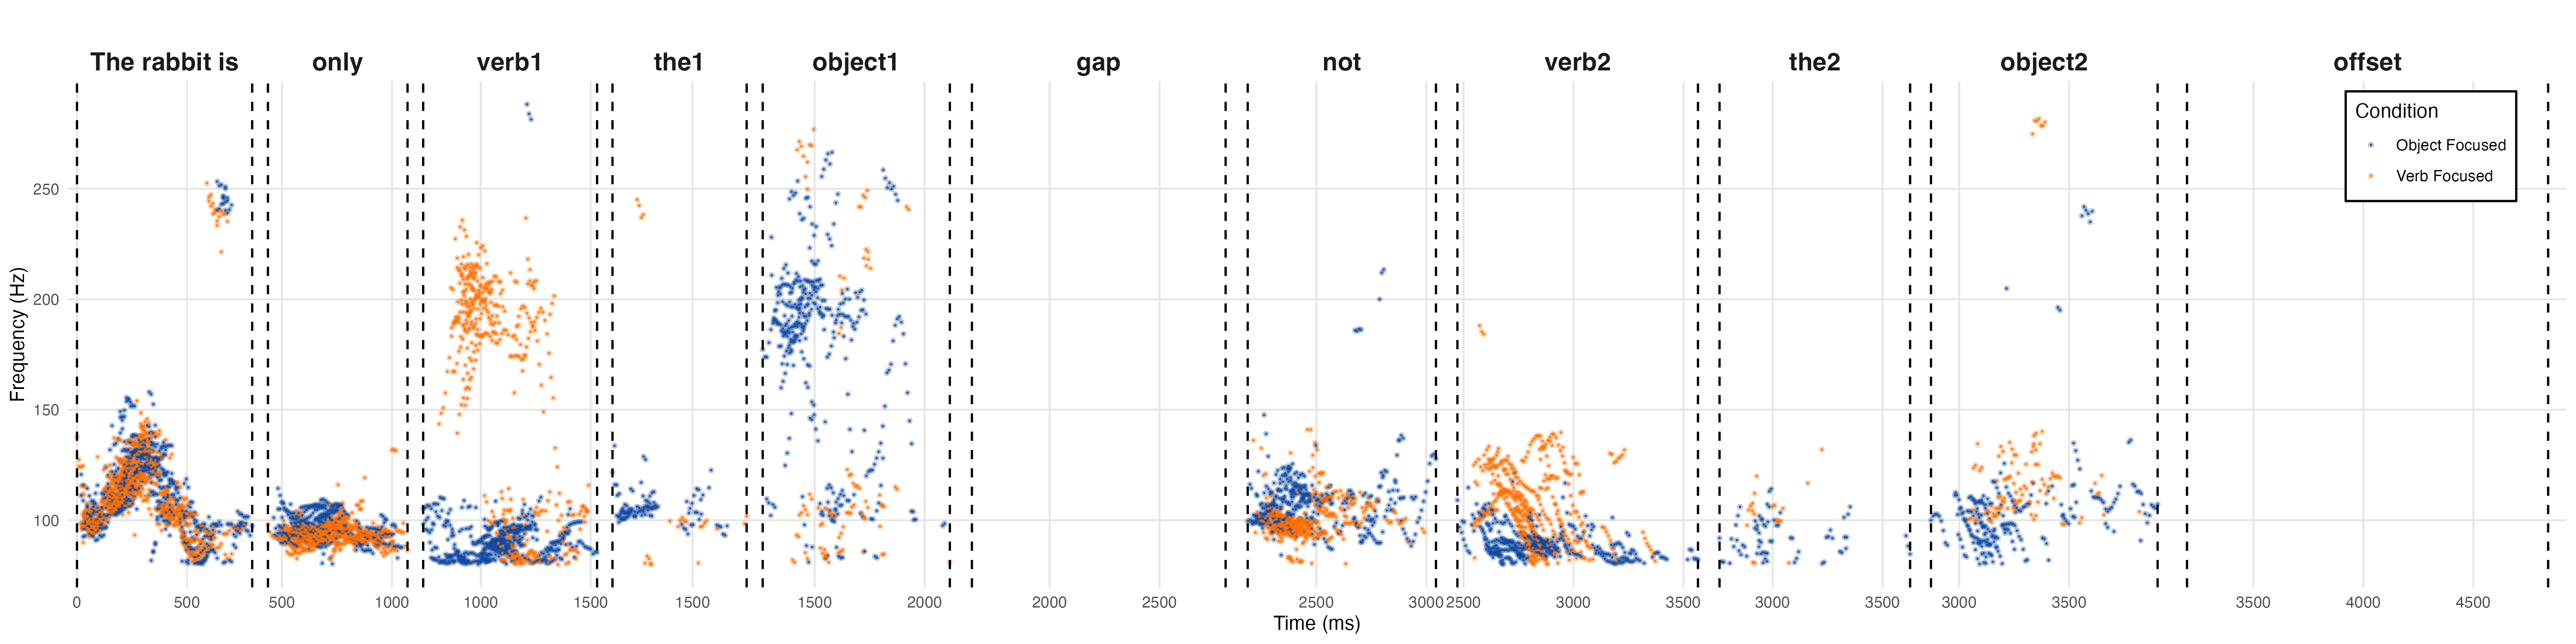
\includegraphics[width=\textwidth,height=\textheight,keepaspectratio]{viz/accoustic.png}
    \caption{Fundamental frequency over time by object-focused (blue) and verb-focused (orange) sentences.}
    \label{fig:acoustic}
\end{figure}



\subsection{Individuals differ in their language processing behavior}
Current experimental evidence suggests that there is a complex interplay between cognitive abilities, auditory perceptual abilities, and motor reproduction abilities during speech processing \parencite{saito2022does, bramlett_wiener_24_speechprosody, bakkouche2025effects, Kachlicka_Saito_Tierney_2019}. Whereas we cannot review (and explore) every possible individual difference predictor, we briefly review five ways in which individuals differ as it relates to spoken language processing: working memory, cognitive control, lexical proficiency, auditory perception abilities, and auditory motor reproduction abilities. These dimensions are theoretically relevant to focus processing because successful integration of prosodic, syntactic, and semantic cues in real time requires flexible cognitive control, precise auditory perception, and potentially sensorimotor alignment for tracking prosodic contours. We therefore include these measures to explore whether individual variability in these domains helps explain differences in how listeners process prosodic focus structure.


\subsubsection{Working memory}
Working memory, or the ability to keep recent input in mind and later draw on it \parencite[see][]{baddeley2003working,carpenter2013role} can affect a wide range of linguistic processes. Based on findings related to working memory and prosody processing research \parencite[e.g.,][]{traxler2009hierarchical,ferreira2015prosody, bishop2021exploring}, the answer most likely depends on the population, task demands, and methods used. For example, working memory, as measured by the digit span task (the same task we use in the present study), was not predictive in terms of identifying English emotional prosody \parencite{sinagra2022perception} or Italian lexical stress \parencite{ppcc} in groups of L1 adults, presumably given the relatively simple task demands of identifying happy/sad prosody or a penultimate/antepenultimate stressed word. How working memory affects the processing of focus prosody in a look-and-listen task is unclear. We use longer sentences involving potential object or verb targets that will require listeners to store linguistic information and draw on it later. (EE2) Do participants with higher working memory show earlier fixations to the focus alternative? If there is an effect of working memory, we assume it will be found among all participants and not just within the L1 or L2 group.


\subsubsection{Cognitive control}
Whereas there are several cognitive tasks used in the psycholinguistics literature \parencite{ness2023state}, we were interested in a task that captures participants' ability to resolve conflict during processing. For this reason, we used the Flanker task \parencite{eriksen1974effects} in which 
participants must focus their attention on congruent stimuli (e.g., $>>>>>$) while resisting attention on incongruent stimuli (e.g., $>><>>$). Congruency tasks such as Flanker have been found to predict behavior in many different linguistic tasks and populations, especially bilinguals who must suppress their L1 while processing their L2 \parencite{blumenfeld2014cognitive,luk2011there} (though see also \cite{hedge2018reliability} for reliability concerns). (EE3) Do L2 speakers with better cognitive control as indexed by performance on the Flanker task show earlier fixations to the focus alternative? If there is an effect of cognitive control, we assume it will be found among only the L2 participants and not the L1 group given the L2 group must suppress their L1 while performing the task.



\subsubsection{Lexical proficiency}
L1 and L2 speakers differ in their lexical proficiency, which has unsurprisingly been shown to contribute to differences in language processing \parencite{Yap2012, zareva2005relationship}. For example, higher lexical proficiency scores are correlated with the speed of activation of the target and the degree to which lexical competition is resolved \parencite{sarrett2022within}. Here, we are interested in whether increased English lexical proficiency, as measured by the LexTALE task \parencite{lemhofer2012introducing}, leads to earlier looks for the L2 English participants. (EE4) Do L2 speakers with greater English proficiency show earlier fixations to the focus alternative? If there is an effect of lexical proficiency, we assume it will be found among only the L2 participants and not the L1 group given the L1 group should have less variation in their English proficiency.

 

\subsubsection{Perceptual auditory sensitivity}
Detecting prosodic cues requires a certain level of sensitivity to the incoming acoustics. Here we look at four measures of what \textcite{saito2023does} calls “explicit acuity in L2 speech learning”: how sensitive a listener is to temporal and spectral cues or dimensions (e.g., formant,
pitch, duration, and intensity). These measures have proven to be reliable measures for a range of L2 speech learning tasks \parencite{Kachlicka_Saito_Tierney_2019, saito2024auditory, bakkouche2025effects, bramlett_wiener_24_speechprosody}. We also know that musical perception ability, which aligns closely with our pitch task, was somewhat predictive of eye fixations \textcite{jansen2023influence}. (EE5) Do speakers with better perceptual auditory sensitivity show earlier fixations to the focus alternative? If there is an effect of auditory sensitivity, we assume it will be found among all participants given that the temporal and spectral cues  that we test---formant, pitch, duration, and intensity---are used in both Dutch and English for focus realization.


\subsubsection{Auditory motor reproduction}
Recent work \parencite{tierney2014auditory, saito2024auditory,tierney2017individual} has argued that motor abilities are a crucial part of auditory processing and that the ability to integrate auditory input to motor actions helps explain various aspects of adult L2 acquisition. We examine whether participants' ability to reproduce target sound sequences for melodies (pitch) and rhythm (duration) is informative for understanding L1 and L2 prosodic processing. (EE6) Do speakers with better auditory motor reproduction show earlier fixations to the focus alternative? If there is an effect of motor reproductions, we assume it will be found among all participants given that this integration ability is necessary for all languages.

\subsection{Motivation for Replicating \textcite{ge2021a}}

We selected Ge et al. (2021a) for replication firstly because the study reported an unexpected L1 Dutch effect in focus processing, where L1 Dutch–L2 English speakers showed sensitivity to prosodic focus that diverged from predictions. Replicating this result was important for testing whether it reflected a robust cross-linguistic effect or a study-specific outcome.

Second, the original study was well documented and thus replicable. The task design and stimuli were described in sufficient detail to permit replication \parencite{mcmanus2024}. At the same time, materials and analysis code were not publicly available, which falls short of emerging norms for reproducible research more broadly \parencite{goodman2016reproducibility} and for eye-tracking specifically \parencite{godfroid2025reporting,AOW}. Because the design was relatively simple and clearly specified, it still provided a suitable baseline for the 
FiREE framework. Moreover, the authors were kind enough to provide the materials when we contacted them. 

Third, the study exemplified the broader challenge of balancing fidelity with the need for more robust analyses and theoretical exploration. It lacked 
acoustic analyses and relied on coarse time-binned models, gaps that align with recent calls for more informative and theory-driven approaches \parencite{xie2023adaptive}. Our replication therefore tested the reliability of the 
original findings while using FiREE to guide refinement and extension.

\subsection{Research Questions}

This study follows the Fidelity, Refinement, and Exploratory Extension (FiREE) framework to structure a layered replication of \textcite{ge2021a}. To guide each phase of the study, we pose the following research questions:

\begin{itemize}
    \item \textbf{RQ1 (Fidelity):} To what extent do we reproduce the key finding from \textcite{ge2021a} that L1 Dutch-L2 English speakers show delayed processing of focus alternatives relative to L1 English speakers?
    
    \item \textbf{RQ2 (Refinement):} To what extent do group differences in focus processing, when analyzed using continuous time-sensitive models (i.e., Generalized Additive Models), emerge as dynamic shifts in fixations over time rather than static processing deficits?
    
    \item \textbf{RQ3 (Exploratory Extension):} To what extent do acoustic features of the stimuli and individual difference measures (e.g., auditory sensitivity, auditory-motor integration, cognitive control, lexical proficiency, working memory) predict changes in target fixations over time during focus processing?
\end{itemize}
